\documentclass[DIV=13,fontsize=11pt]{scrartcl}
\usepackage[T1]{fontenc}
\usepackage{lmodern}
\usepackage[ngerman]{babel}
\usepackage[utf8]{inputenc}
\usepackage{csquotes}
\usepackage[hidelinks]{hyperref}
\usepackage{amsmath}
\usepackage{amssymb} 
\usepackage{listings}
\usepackage{float}
\usepackage{dirtree}
\usepackage{booktabs}
\usepackage{graphics,graphicx}
\usepackage[left=2cm, right=2cm, top=2cm, bottom=2cm, bindingoffset=1cm, includeheadfoot]{geometry}
\usepackage[onehalfspacing]{setspace}
\usepackage{pdfpages}
\usepackage[backend=biber,style=numeric,maxcitenames=1,sorting=none]{biblatex}\addbibresource{bib.bib}

% aendert u.a. bei zitierungen zu et al.
\DefineBibliographyStrings{ngerman}{ 
   andothers = {et\addabbrvspace al\adddot},
   andmore   = {et\addabbrvspace al\adddot},
}

\setlength{\parindent}{0pt}

\begin{document}
% ----------------------------------------------------------------------------
\subject{Projektbericht zum Modul Data Mining Wintersemester 20221/2022}
\title{Reproduktion des Papers \\ \textit{Context-Sensitive Visualization of Deep Learning Natural Language Processing Models}\cite{dunn2021context}}
\author{Max Henze}% obligatorisch
\maketitle% verwendet die zuvor gemachte Angaben zur Gestaltung eines Titels
% ----------------------------------------------------------------------------

\section{Einleitung}
% Beitrag Originalartikel: bessere Visualisierung von Wortwichtigkeit bei Klassifizierung durch Transformer Neural Network
% bearbeitete Teile: alle ( LNO Algorithmus und zusätzlich eigenes BERT Modell) 
% neue Erkenntnisse: 
% eigener Beitrag: Code zum Originalartikel, da keiner vorhanden 

Neuronale Netzwerke sind ein beliebtes Hilfsmittel im Bereich von NLP.
Besonders Modelle, welche sich mit dem Einsatz von Transformern,
wie BERT~\cite{devlin2018bert} oder GPT-2~\cite{radford2019language}, behelfen,
gehören schon lange zum state-of-the-art. Doch diese Modelle mit ihrer
Vielzahl an Layern, Neuronen und Verbindungen, gewähren einen nicht
gerade einfachen Einblick in ihre Verarbeitungsschritte. Ansätze wie Leave-One-Out
oder Leave-N-Out versuchen durch Neuklassifikation von modifizierten Texten einen
allgemeinen Einblick in die Verarbeitungsstrukturen von Neuronalen Netzwerken zu geben.
Diese Ansätze betrachten aber nicht einen möglichen Kontext, wie er zwischen
Wörtern in einem Satz existieren kann.
\citeauthor{dunn2021context} haben daher in ihrem Artikel \citetitle{dunn2021context}
eine Methode entwickelt, um Wörter mit ihrer unterschiedlichen Wichtigkeitsgewichtung
innerhalb der Klassifizierung und unter Inbetrachtnahme von Kontexten zu visualisieren.
Als Replikationsziel wurde für diese Arbeit der gesamte Visualisierungsprozess
von \citeauthor{dunn2021context} gewählt. Zusätzlich dazu wurde ein eigenes
BERT Modell auf dem gegebenen IMDB~\cite{maas-EtAl:2011:ACL-HLT2011} Datensatz trainiert, um
dieses für den späteren Klassifikationsprozess zu verwenden. Darüber hinaus
wurden zwei zusätzliche Methodiken zur Visualisierung mit Kontexten überprüft,
welche in ihrer Effektivität jedoch hinter der von \citeauthor{dunn2021context}
stehen.
Durch die Replikation wird eine verständliche Codebeigabe zum Originalartikel
erzeugt, welche dem Leser ein noch besseres Verständnis liefern soll. So können
mit dem System alle Dokumente des Testdatensatzes klassifiziert und visualisiert werden
um so eine größere Vielfalt von Beispielen und ein besseres Verständnis bereitzustellen.

\section{Umfang der Replikation/Reproduktion}
% Behauptung/Hypothese: bessere Visualisierung von Wortwichtigkeit durch leve-n-out mit abhängigen Wörtern

Als Ziel dieser Replikation wurde die einzige Hypothese gewählt, welche
\citeauthor{dunn2021context} in ihrem Artikel behandeln. Sie propagieren,
dass sich die Wichtigkeit eines Wortes innerhalb der Klassifikation durch ein
Neuronales Netzwerk anhand des durch den Vergleichs der sogenannten
Prediction Strength (Sicherheit des NN, dass Label richtig klassifiziert ist)
des Originaltextes zur Pediction Strength des Textes ohne das betrachtete Wort (Leave-One-Out)
ergibt. Ebenfalls ist der Einbezug von kontextuell zusammhängenden Wörtern (Leave-N-Out)
für die Autoren wichtig. \glqq Unser Ansatz schaut auf die Kombination von
Wörtern und Sätzen, um deren Einfluss auf die Ausgabe des Modells zu erkennen,
was zu einer Visualisierung führt, welche kontextsensitiver zum Originaltext ist.
\grqq~\cite{dunn2021context}\\

Somit ist folgende Behauptung das Ziel dieser Replikation:

\begin{itemize}
    \item Der Leave-N-Out Ansatz ist geeigneter bei der Erkennung kontextueller Wörter und Strukturen als der des Leave-One-Out.
\end{itemize}

\section{Methoden}

Die Replikation des Originalartikels ergibt sich wie folgt. Durch die
fehlende Beigabe von Code mussten alle Ideen und Modelle von \citeauthor{dunn2021context}
eigenständig implementiert werden. Dazu wurde sich an Wortangaben
der Autoren wie zum Beispiel:
\glqq Der gesamte Code ist geschrieben in Python 3.8 und nutzt die Tensorflow Version
der Transformersbibliothek. [...] Texttokenisierung und Abhängigkeitsbestimmung wurden
mit der spaCy NLP Bibliothek durchgeführt.\grqq~\cite{dunn2021context} gehalten.\\

Zur Klassifizierung von Dokumenten wurde ein Modell unter der Verwendung von BERT trainiert.
Da keine weiteren Angaben zu finden waren und eine große Auswahl an unterschiedlichen
BERT Modellen zu finden ist wurde das \textit{BERT uncased L-12 H-768 A-12} Modell gewählt.
Dieses zählt auf Tensorflow Hub\footnote{\url{https://tfhub.dev}} zu den am häufigsten verwendeten
BERT Modellen (über 214.000 Downloads).\\

Entwickelt wurde innerhalb eines Jupyter Notebooks mit Python.
Die folgenden essentiellen Packages fanden dabei Anwendung:

\begin{figure}[H]
    \centering
    \begin{tabular}{ll}
        \toprule
        Package Name    & Package Funktion                             \\
        \midrule
        tensorflow\_hub & Einbindung des BERT Modells                  \\
        tensorflow      & Modellerzeugung und Training                 \\
        official.nlp    & Trainingsoptimisierung                       \\
        spacy           & Abhängigkeitsbestimmung (Dependency Parsing) \\
        pandas          & Arbeiten mit Dataframes                      \\
        matplotlib      & Visualisierung der Texte                     \\
        \bottomrule
    \end{tabular}
    \caption{Verwendete Packages}
    \label{fig:packages}
\end{figure}

Das BERT Modell wurde auf einer Nvidia Geforce RTX 3070 mit 8 GB Arbeitsspeicher
trainiert.

\subsection{Modellbeschreibung}

Innerhalb des Originalartikels sind keine Angaben bezüglich der Zielfunktion und
Parameter zu finden. Angaben zum Modell beruhen auf der Benennung eines BERT Modells und
einer Modellbeschreibung, welche auf das Anhängen eines Dropout-Layers und
Dense-Layers verweist.\\

Die beschriebene Methodik ist wie folgt:\\

Ein Text wird durch das Modell klassifiziert und die damit korrespondierende
Ausgabestärke, der Score, notiert. Nun werden mit Hilfe einer Abhängigkeitsbestimmung
alle Beziehungen zwischen Wörtern aufgedeckt. Anschließend werden neue Texte
erzeugt, in denen jeweils ein Wortpaar, welches eine Verbindung zueinander
aufweist, entfernt wurde. Das Modell klassifiziert die nun
erhaltene Sammlung an neuen Texten und vergleicht die neuen Ausgabestärken mit der des
Ausgangstextes. Texte mit größeren oder gleichen Ausgabestärken
als der des Originals tragen scheinbar nicht zur Klassifikation bei und werden
entfernt. Dies geht mit unserer Intuition einher wie das folgende Beispiel erklärt.\\

Nehmen wir an, der Satz \textit{I love this film so much.} wurde durch das Modell mit
einem Score von 0.9 bewertet. Das Neuronale Netzwerk ist sich somit sehr sicher,
dass dieser Satz das Label eins, also positiv, bekommen sollte. Würden wir den Text
folgendermaßen modifizieren: \textit{I love film so much.} und das Modell
nun einen Score von 0.95 vergeben, würde durch das Weglassen von \textit{this} die
Sicherheit, dass es sich hier um ein positives Label handelt, steigen.
Somit lässt sich annehmen, dass \textit{this} keinen Beitrag zur Klassifikation
des Labels leistet. Dementsprechend können wir es aus unseren Betrachtungen entfernen.\\

Je größer nun eine Differenz ist, umso wichtiger ist das
Wortpaar für die Klassifizierung. Mit Hilfe einer Linearisierung der Differenzen
und einer Colormap können Wörter somit bezüglich ihrer Wichtigkeit
farblich kenntlich gemacht werden. Je wichtiger umso grüner, je unwichtiger, desto blauer.

\subsection{Datenbeschreibung}

\begin{figure}[H]
    \centering
    \begin{minipage}{5cm}
        \dirtree{%
            .1 data.
            .2 test.
            .3 neg.
            .4 x\_y.txt.
            .4 ....
            .3 pos.
            .4 x\_y.txt.
            .4 ....
            .2 train.
            .3 neg.
            .4 x\_y.txt.
            .4 ....
            .3 pos.
            .4 x\_y.txt.
            .4 ....
        }
    \end{minipage}
    \caption{Ordnerstruktur des Datensatzes. x ist die Dokumenten-Id und y ist eine Sternewertung von Null bis Zehn.}
    \label{fig:filestruc}
\end{figure}

Der im Originalartikel und dieser Replikation verwendete Datensatz ist das Large Movie
Review Dataset~\cite{maas-EtAl:2011:ACL-HLT2011} der Universität Stanford.
Dieser umfasst 50.000 Dokumente, darunter 25.000 Trainingsdokumente und 25.000 Testdokumente. Er ist unter
\url{https://ai.stanford.edu/~amaas/data/sentiment/} verfügbar.\\

Der Datensatz hat eine vorgegebene Ordnerstruktur, siehe Abbildung \ref{fig:filestruc}.
So befinden sich die Trainings- und Testdokumente in eigenen Ordnern,
wobei positive und negative Dokumente nochmals in eigene Ordner unterteilt sind.
Die Dokumente unterscheiden sich stark in der Länge. So gibt es Dokumente mit knapp über 50,
aber auch solche mit über 13.000 Zeichen.
Die Dokumente an sich sind nicht aufbereitet, enthalten englische Alltagssprache und Sonderzeichen.

\begin{figure}[H]
    \centering
    \begin{lstlisting}
        Fair drama/love story movie that focuses on the lives of 
        blue collar people finding new life thru new love.The acting 
        here is good but the film fails in cinematography,screenplay,
        directing and editing.The story/script is only average at best.
        This film will be enjoyed by Fonda and De Niro fans and by 
        people who love middle age love stories where in the coartship 
        is on a more wiser and cautious level.
        It would also be interesting for people who are 
        interested on the subject matter regarding illiteracy.......
    \end{lstlisting}
    \caption{Beispieltext eines positiven Trainingsdokuments}
\end{figure}

Bei der Verwendung der Daten zum Training des Modells, wurde der Trainings- zusätzlich in einen
Validierungsdatensatz aufgeteilt. Dieser umfasst 20 Prozent der Trainingsdaten und somit 5.000 Dokumente.

\subsection{Hyperparameter}

Folgende Hyperparameter wurden gesetzt:

\begin{figure}[H]
    \centering
    \begin{tabular}{ll}
        \toprule
        Parameter    & Wert \\
        \midrule
        Batch Size   & 16   \\
        Epochs       & 1    \\
        Learningrate & 3e-5 \\
        Dropoutrate  & 10\% \\
        \bottomrule
    \end{tabular}
\end{figure}

Die Batch Size definiert die Menge an Trainingsdaten, welche vom Netzwerk auf einmal
verarbeitet werden bevor es sich aktualisiert. Diese wurde auf 16 festgesetzt, da das
Modell auf der zuvor schon erwähnten Nvidia Grafikkarte trainiert werden sollte.
Größere Batch Sizes haben sich als Problem entpuppt, da diese nicht mehr in den
Speicher passten.
Bei der Epochenanzahl wurde nur eine festgelegt.
Beginnend lag dieser Wert bei fünf. Doch verschiedene Durchläufe und eine Einbindung
von Early Stopping ergaben, dass das Modell nach der ersten Epoche die
beste Leistung aufwies. Mit zunehmendem Training stieg auf dem Trainingsdatensatz
die Accuracy und im selben Moment sank der Loss. Dahingegen stieg auf dem Validierungsdatensatz
der Loss bei gleichbleibener Accuracy in jeder Epoche. Dies war ein eindeutiges
Zeichen für Overfitting.

\subsection{Implementierung}

Der Code zur Implementierung ist abrufbar unter: \url{https://github.com/maxhenze/Klausurleistung.git}
Die wichtigsten verwendeten Packages finden sich in Abbildung \ref{fig:packages}.\\

Durch die Verwendung eines Jupyter Notebooks ist der Code interaktiv gehalten.
Parameter können angepasst und dadurch erzeugte Modelle sofort
neu trainiert werden, falls die Hardware dies zulässt. Falls nicht
sind im Projekt zwei fertige Modelle vorhanden, welche eigenständig trainiert wurden.\\

Diese können im Notebook geladen und verwendet werden. Es muss durch einen
entsprechenden Flag gesetzt werden, ob ein Modell trainiert oder geladen werden soll.
Je nachdem werden ungebrauchte Codeteile übersprungen.\\

Der Datensatz wird automatisch heruntergeladen und entpackt, je nachdem, ob
Daten schon vorhanden sind.\\

Die Einteilung der Trainingsdaten in Trainings- und Validierungsmenge wird durch
einen Seed bestimmt. Durch unterschiedliches Setzen werden verschiedene
Daten zum Training bzw. zur Validierung benutzt. Hauptsächlich ist dieser
Wert aber dazu da, damit kein Dokument in beiden Datensätzen auftaucht.\\

Ein anderes BERT Modell kann ebenfalls geladen werden. Dazu muss nur der passende
Link von Tensorflow Hub für die Variable \texttt{tfhub\_handle\_encoder} ersetzt
werden.\\

Bei dem zuvor schon erwähnten Optimierer handelt es sich um den AdamW~\cite{DBLP:journals/corr/abs-1711-05101}
Optimierer, welcher die Parameter des Modells dynamisch während des Lernprozesses
anpasst.\\

\subsection{Aufbau der Experimente}

Zur Durchführung der Experimente des Originalartikels wurden die Dokumente
aus der Testdatenmenge verwendet. Eine Zelle des Notebooks hat dabei die Aufgabe ein zufälliges
Dokument zu wählen. Durch das Nacheinanderausführen der dahinter liegenden
Zellen werden die Klassifikations- und weiteren Rechenschritte zur Visualisierung
automatisch abgearbeitet. Am Ende erhält man ein fertiges Bild des
eingefärbten Textes. Dabei wird auf der einen Seite der Leave-One-Out und auf der
anderen der Leave-N-Out Ansatz durchlaufen, so dass am Ende zwei Texte herauskommen,
welche miteinander verglichen werden können.

\section{Ergebnisse}

\subsection{Ergebnis 1}

\begin{figure}[H]
    \centering
    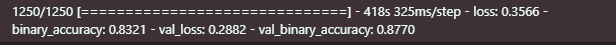
\includegraphics[width=\linewidth]{img/train_time.png}
    \caption{Trainingsergebnisse des Klassifikationsmodells mit BERT und angehängtem Dropout und Dense Layer.}
    \label{fig:modell_train}
\end{figure}

\begin{figure}[H]
    \centering
    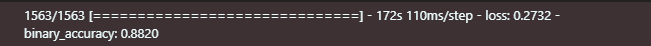
\includegraphics[width=\linewidth]{img/test_time.png}
    \caption{Testergebnisse des Klassifikationsmodells mit BERT und angehängtem Dropout und Dense Layer.}
    \label{fig:modell_test}
\end{figure}

Die Replikation des Klassifikationsmodells ergab nach einer Trainingsepoche ein Modell mit einer Accuracy von $0.877$ und
einem Loss von $0.2882$. Es wird also ein Großteil der Daten richtig klassifiziert. Diese Ergebnisse konnten innerhalb
der Testdaten bestätigt werden, siehe Abbildung \ref{fig:modell_train} und \ref{fig:modell_test}.

Das Training mit größerer Epochenanzahl ergab keine Verbesserung der Acurracy, aber einer Steigerung des Losses. Dies
deutet auf Overfitting hin.

\subsection{Ergebnis 2}

Die Ergebnisse des Originalartikels konnten durch die Replikation bestätigt werden. Leichte Abweichungen
ergaben sich in der genauen Einfärbung der Wörter. Dies lässt sich auf ein unterschiedliches Klassifikationsmodell,
welches leicht abweichende Werte produziert oder ein abweichendes Farbschema zurückführen.
Ebenso gibt es Beispiele des Originalartikels, welche falsch vom Modell klassifiziert werden.\\

Die folgenden Beispiele sind dieselben wie im Orginialartikel, welche
jeweils mit dem Leave-One-Out und Leave-N-Out Ansatz visualisiert wurden.

\begin{figure}[H]
    \centering
    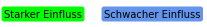
\includegraphics[]{img/legend.png}\\
    Leave-One-Out\\
    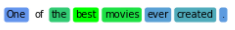
\includegraphics[]{img/first_ex_loo.png}\\
    Leave-N-Out\\
    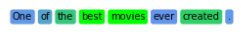
\includegraphics[]{img/first_ex_lno.png}
    \caption{Wie im Originalartikel wurde hier mit dem Leave-N-Out der Zusammenhang von \textit{best} und \textit{movies} besser gekennzeichnet. Im Gegensatz zum Originalartikel, wurde hier bei beiden das Wort \textit{created} als beeinflussend gekennzeichnet.}
    \label{fig:ex1}
\end{figure}

\begin{figure}[H]
    \centering
    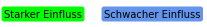
\includegraphics[]{img/legend.png}\\
    Leave-One-Out\\
    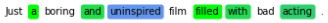
\includegraphics[]{img/sec_ex_loo.png}\\
    Leave-N-Out\\
    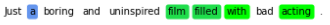
\includegraphics[]{img/sec_ex_lno.png}
    \caption{In diesem Beispiel konnten die kontextuellen Zusammenhänge von \textit{boring} und \textit{film}, sowie \textit{bad} und \textit{acting} durch den Leave-N-Out Ansatz besser verdeutlicht werden.}
    \label{fig:ex2}
\end{figure}

\begin{figure}[H]
    \centering
    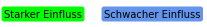
\includegraphics[]{img/legend.png}\\
    Leave-One-Out\\
    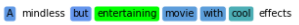
\includegraphics[]{img/third_ex_loo.png}\\
    Leave-N-Out\\
    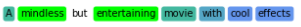
\includegraphics[]{img/third_ex_lno.png}
    \caption{Auch in diesem Beispiel findet sich eine Übereinstimmung zum Originalartikel. \textit{mindless} wird hier mit \textit{entertaining} stärker in Beziehung gesetzt.}
    \label{fig:ex3}
\end{figure}

\begin{figure}[H]
    \centering
    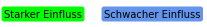
\includegraphics[]{img/legend.png}\\
    Leave-One-Out\\
    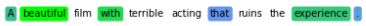
\includegraphics[]{img/fourth_ex_loo.png}\\
    Leave-N-Out\\
    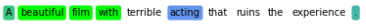
\includegraphics[]{img/fourth_ex_lno.png}
    \caption{Dieses Beispiel bietet gar keine Übereinstimmung mit dem Originalartikel. \textit{terrible} und \textit{ruins} werden gar nicht in Betracht gezogen. Der Fehler scheint hier beim Modell zu liegen. Es klassifiziert bei diesem Beispiel das falsche Label. Vermutlich aufgrund der Einleitung mit \textit{a beautiful film}.}
    \label{fig:ex4}
\end{figure}

Wie in den Abbildungen \ref{fig:ex1} bis \ref{fig:ex3} zu sehen ist, sind die Ergebnisse nahezu äquivalent zu denen des
Originalartikels. Bei denen, wo das Klassifikationsmodell richtig liegt, lässt sich auch die
spätere Visualisierung des Originalartikels in leicht abweichenden Farbnuancen replizieren.
Das Experiment, in dem das Modell schon im Vorhinein scheitert, siehe Abbildung \ref{fig:ex4}, ergibt auch eine stark abweichende Visualisierung.

\begin{figure}[H]
    \centering
    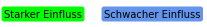
\includegraphics[]{img/legend.png}\\
    Leave-One-Out\\
    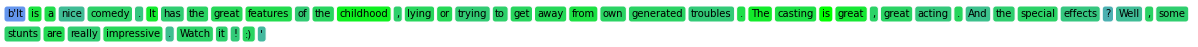
\includegraphics[width=\linewidth]{img/new_ex1_loo.png}\\
    Leave-N-Out\\
    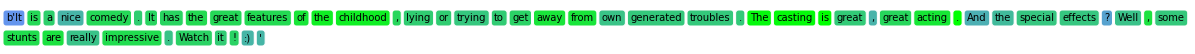
\includegraphics[width=\linewidth]{img/new_ex1_lno.png}
    \caption{Vergleich längerer Texte. Veränderte Einflüsse fallen hier nur in Nuancen auf.}
    \label{fig:ex5}
\end{figure}

Bei längeren Texten fallen die veränderten Zusammenhänge nicht sofort auf. Jedoch ist auffällig, dass bei längeren Texten
oft nur einzelne Wörter vom Modell als wichtig interpretiert werden. Dadurch ergeben sich Visualisierungen wie in Abbildung \ref{fig:ex6}.

\begin{figure}[H]
    \centering
    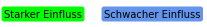
\includegraphics[]{img/legend.png}\\
    Leave-N-Out\\
    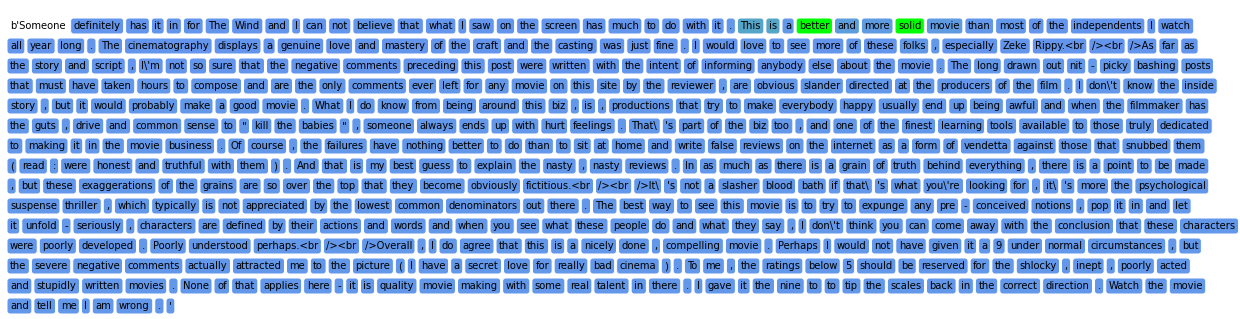
\includegraphics[width=\linewidth]{img/long_ex_lno.png}
    \caption{Visualisierung langer Texte. Einzelne Wörter fallen hier stark ins Gewicht, wohingegen alle anderen Wörter als nicht stark beeinflussend gekennzeichnet werden.}
    \label{fig:ex6}
\end{figure}

\subsection{Zusätzliche Ergebnisse, die nicht im Originalartikel enthalten waren}

Zusätzlich zu den Experimenten des Originalartikels wurde zwei weitere Methodiken des Leave-N-Out Ansatzes implementiert.\\

Ersteres versucht das Weglassen eines Elternwortes mit allen von ihm abhängigen Kindern. Dabei wird deutlich, dass
hierbei zu viele Wörter entfernt werden, wodurch Abhängigkeiten schlechter dargestellt werden. Diese Methodik
ähnelt in der Visualisierung stark der Leave-One-Out Methodik.\\

Letzteres hingegen versucht, zusätzlich zum Elternwort alle Nachfahren dieses Wortes wegzulassen. Somit werden auch
implizite Verbindungen von Wörtern in Betracht gezogen, welche nicht durch eine direkte Abhängigkeit miteinander
verbunden sind. Diese Methodik erzeugt ähnliche Darstellungen wie die Leave-N-Out Methodik des
Originalartikels, wobei direkte Abhängigkeiten etwas schwächer visualisiert werden. Indirekte werden
hingegen hervorgehoben, wodurch größere Teilabschnitte bzgl. der Farbgebung zusammengefasst werden.
Dies ist sichtbar in Abbildung \ref{fig:ex7}.

\begin{figure}[H]
    \centering
    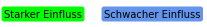
\includegraphics[]{img/legend.png}\\
    Leave-N-Out\\
    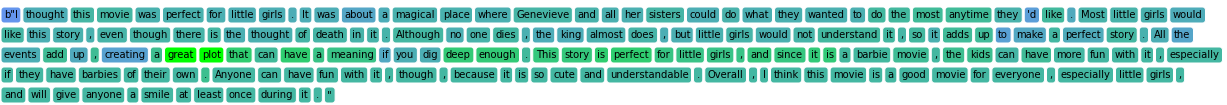
\includegraphics[width=\linewidth]{img/own_ex_lno.png}\\
    Leave-Ancestors-Out\\
    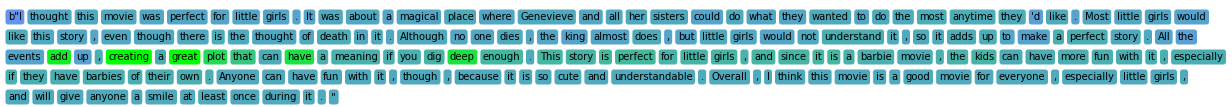
\includegraphics[width=\linewidth]{img/own_ex_lao.png}\\
    Leave-One-Out\\
    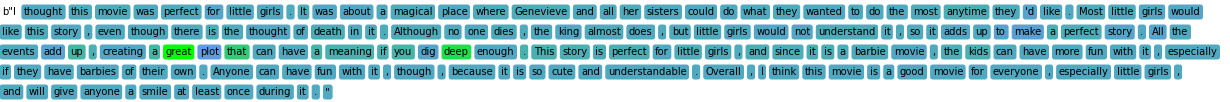
\includegraphics[width=\linewidth]{img/own_ex_loo.png}\\
    Leave-Children-Out\\
    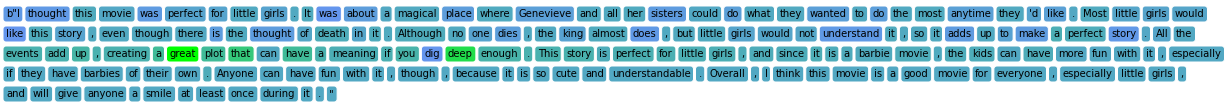
\includegraphics[width=\linewidth]{img/own_ex_lco.png}\\
    \caption{Visualisierung eines Textes mit zusätzlich erdachten Methodiken. In dieser Abbildung werden die Methodiken der Leave-N-Out und Leave-One-Out des Originalartikels mit den selbsterdachten Methodiken Leave-Ancestors-Out und Leave-Children-Out verglichen.}
    \label{fig:ex7}
\end{figure}


\section{Diskussion}
Der im Originalartikel propagierte Leave-N-Out Ansatz schafft es im Vergleich zum Leave-One-Out Ansatz, kontextuell abhängige
Wörter bei der Visualisierung besser in Bezug zu setzen. Die hier zu stellende Frage ist, ob die dadurch in Bezug gesetzten Wörter einen besseren
Einblick in die Klassifikation eines Neuronalen Netzwerkes ermöglicht ? Natürlich ist es bei Sätzen wie \textit{One of the best movies ever created.} richtig,
dass die Wörter \textit{best} und \textit{movie} durch ihren kontextuellen Zusammenhang eine gleichwertige Wichtigkeitsgewichtung erhalten sollten.
Dennoch wird durch den Leave-One-Out Ansatz deutlich, dass das Neuronale Netzwerk das Wort \textit{best} stärker für die Klassifizierung benutzt
als das Wort \textit{movies}. Dies gibt eine stärkere Einsicht in die Wichtigkeit eines einzelnen Wortes. Beim Leave-N-Out Ansatz hingegen
ist unklar, ob durch das Weglassen beider Wörter  oder nur durch das Weglassen des stärker klassifizierten Wortes die Klassifizierung schlechter geworden ist.\\

Der Originalartikel war trotz fehlenden Codes replizierbar. Die Aussagen der Autoren gaben einen guten Einblick in die verwendeten Strukturen und Techniken,
welche mit Hilfe von state-of-the-art Modellen gut umgesetzt werden konnten. Dennoch sind leichte Abweichungen, durch fehlende Angaben zum
BERT Modell, vorhanden. Ebenso ist eine abweichende Farbskala ein ebenso möglicher Grund für leicht verschiedene Darstellungen.\\

Es wurde deutlich, dass der Originalansatz im Vergleich zu den selbst dargestellten Methodiken eine bessere Visualisierung von kontextuell
abhängigen Wörtern ermöglicht.

\subsection{Was war einfach?}
Aufgrund des recht einfachen, propagierten Ansatzes, waren nahezu alle Umsetzungen der Leave-N-Out Methodik nicht schwer zu implementieren.
Durch klare Package Benennung und einer einfachen Algorithmusbeschreibung konnten alle Schritte von der Klassifikation, dem Produzieren neuer Texte,
der Filterung der Neuklassifikation und der Visualisierung problemlos repliziert werden. So benötigte das Einlesen in die API des jeweiligen
Packages eine gewisse Zeit, dennoch handelte es sich dabei nie um zu umfängliche Beschreibungen.\\

Das angegebene spacy Package ist ein sehr gutes Tool für die Erstellung von Abhängigkeitsgraphen, auf denen sich recht
einfach navigieren lässt, wodurch die Abhängigkeitsbestimmung dadurch auch nicht besonders schwer viel. Und die Bearbeitung
auf den neu generierten Texten fiel ebenfalls, durch das sehr umfängliche pandas Package, sehr leicht aus.

\subsection{Was war schwer?}
Die Implementierung des Klassifikationsmodells sowie der allgemeine Umgang mit diesem war nicht sehr einfach.
Durch fehlende Angaben der Autoren zum Modell war beginnend eine gewisse Recherche notwendig, welches BERT Modell nun genau
benutzt werden soll. Es wurde zwar grob eine Implementierung der verschiedenen Layer erwähnt, diese war aber nicht ausreichend
für die eigenständige Erstellung. Angaben der Daten waren ebenfalls recht sporadisch, wodurch erst eine geeignete Implementationsstruktur
erdacht werden musste. Auch die Tatsache, dass keine Angaben zu Hyperparametern gemacht wurden, trug erschwerend bei. Das Finden der richtigen
Batch Size und das Einstellen des Trainings auf der Grafikkarte erwies sich als äußert umständlich, da zu große Batch Sizes für einen
\texttt{Out Of Memory} Error sorgten und das Training auf einer CPU (8 Kerne) dennoch zu langsam war.

\subsection{Empfehlungen für die Replizierbarkeit}
Natürlich wäre ein, von vornherein beigereichter, Code sehr praktisch gewesen. Wobei sich auch hier sagen lässt, dass das Verstehen von
fremdem Code eine Problematik in sich ist. Genauere Angaben zur Implementierung würden hier schon reichen. Eine genaue Angabe des verwendeten
BERT Modells sowie eine Bereicherung der verwendeten Hyperparameter und einer Hardwarebeschreibung würde viel Testen obsolet machen.
Zusätzlich dazu, auch wenn nicht unbedingt von Nöten, wäre eine Angabe von verwendeten Funktionen der Packages, welche zur Realisierung
des Algorithmus verwendet wurden, sehr bequem.

\section{Kommunikation mit den Autoren}

\section{Anhang}

\subsection{Notebook Code}

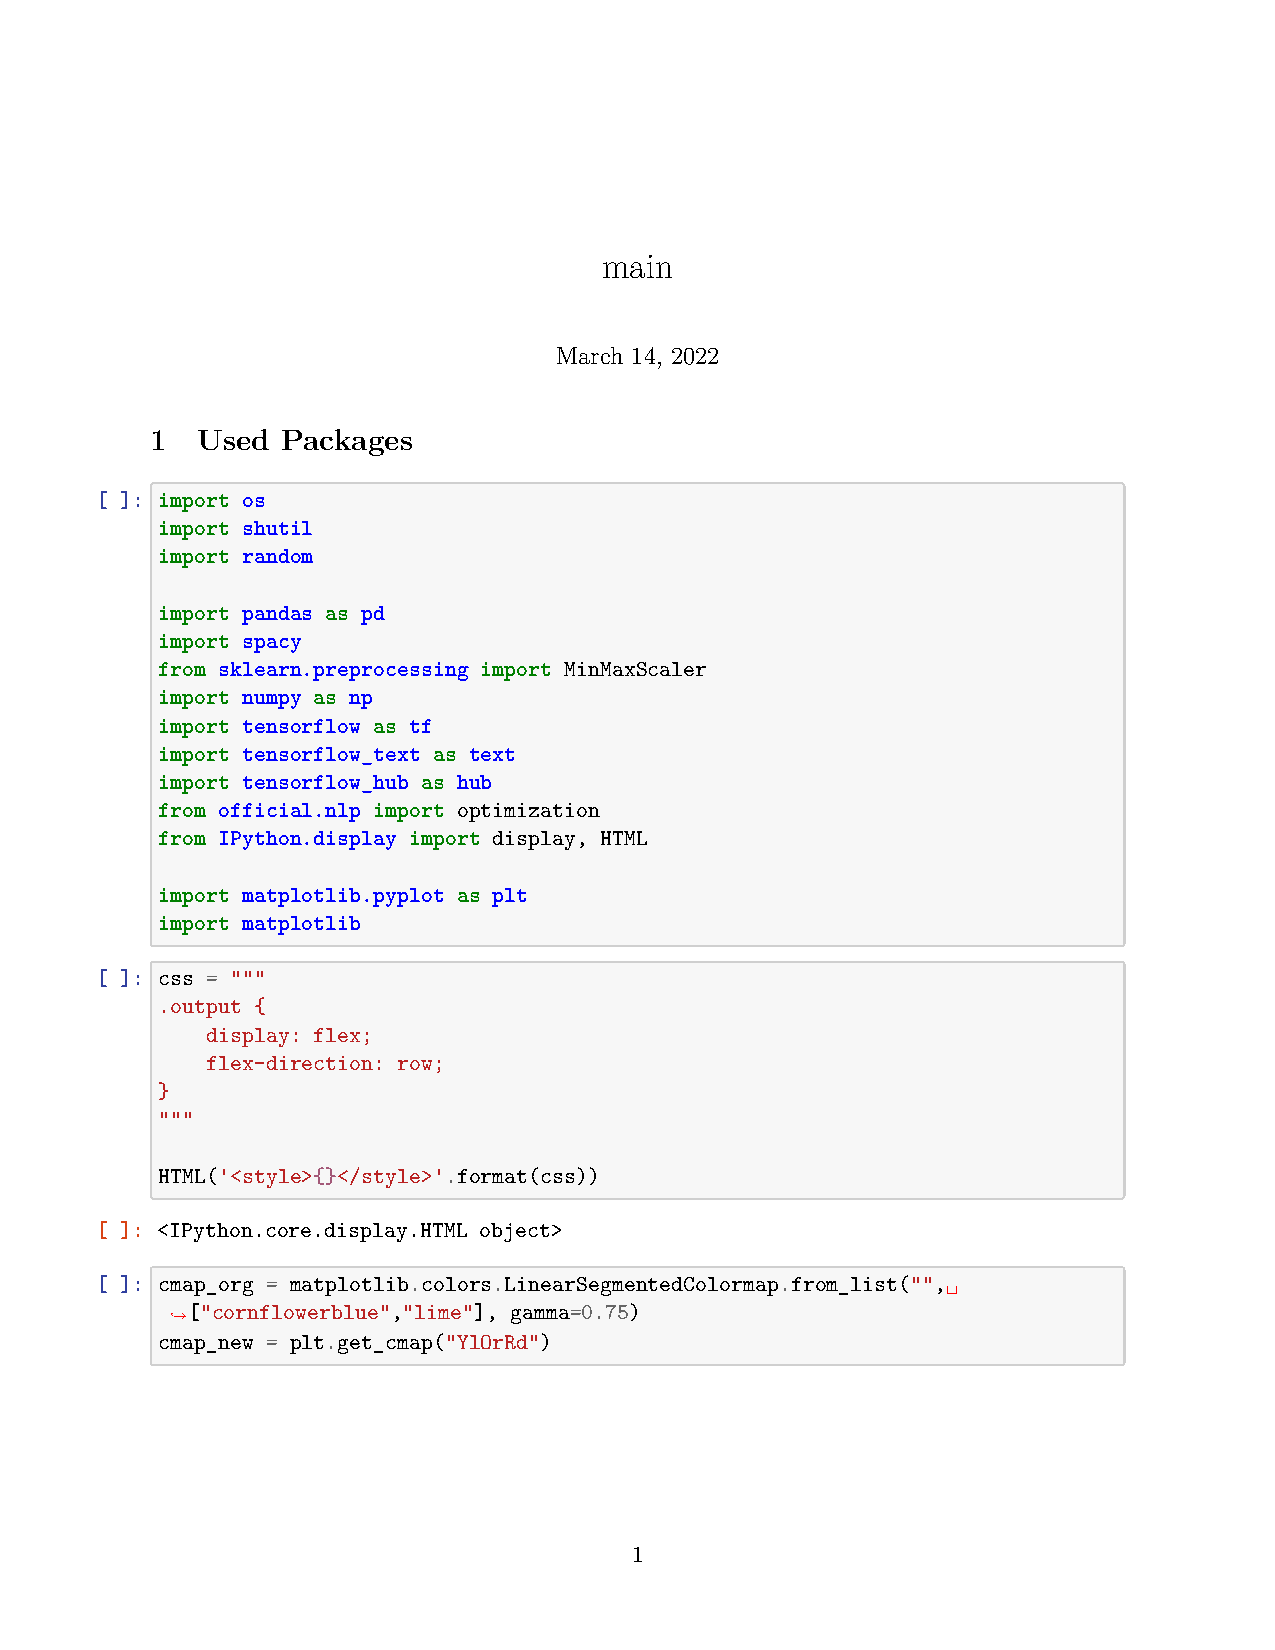
\includepdf[pages=-, pagecommand={\thispagestyle{empty}}]{pdf/project.pdf}

\subsection{Git-Historie}
\begin{figure}[H]
    \tiny
    \begin{lstlisting}
        * 65ddb6a (HEAD -> master, origin/master) (added minor changes to article, 2022-03-14)
        * 5997180 (Exported project to html and pdf, 2022-03-14)
        * 787d109 (added all sections up to communication with autors, 2022-03-11)
        * c9035db (Added additional Experiments, 2022-03-09)
        * 01fe9ee (changed structure, capsuled certain calls in functions, 2022-03-09)
        * 0763df8 (added further text in example section, 2022-03-07)
        * e13b3cc (Corrected calculations for negative labels, 2022-03-07)
        * 1743a87 (added examples and wrote text furhter, 2022-03-04)
        * f358118 (overhauled paper texts up to hyperparameter, 2022-03-04)
        * 8623038 (added leave n out experiment, 2022-03-04)
        * 49ad312 (changed notebook (cont), 2022-03-02)
        * b0e9404 (added new (better) model , startet writing report, changed notebook structure, 2022-03-02)
        * 614af17 (updated gitignore, 2022-03-02)
        * 70efdb4 (added report framework, 2022-03-02)
        * ad222c3 (Better visualization, custom cmap, 2022-02-24)
        * f49b4c9 (Added text visualization, 2022-02-24)
        * cdc060f (Commit with trained Model, dependency parsing and leave n out, 2022-02-23)
        * 959dcb1 (Add lfs support, 2022-02-23)                
    \end{lstlisting}
\end{figure}
\printbibliography

\end{document}
